% !TEX root = ../slides_ISSTA.tex


\begin{frame}
\frametitle{What is a Regular Expression?}

example

\end{frame}
%------------------------------------------------

\begin{frame}
\frametitle{In Python: Utilizations of the re module}
\begin{figure}[h]
  \centering
  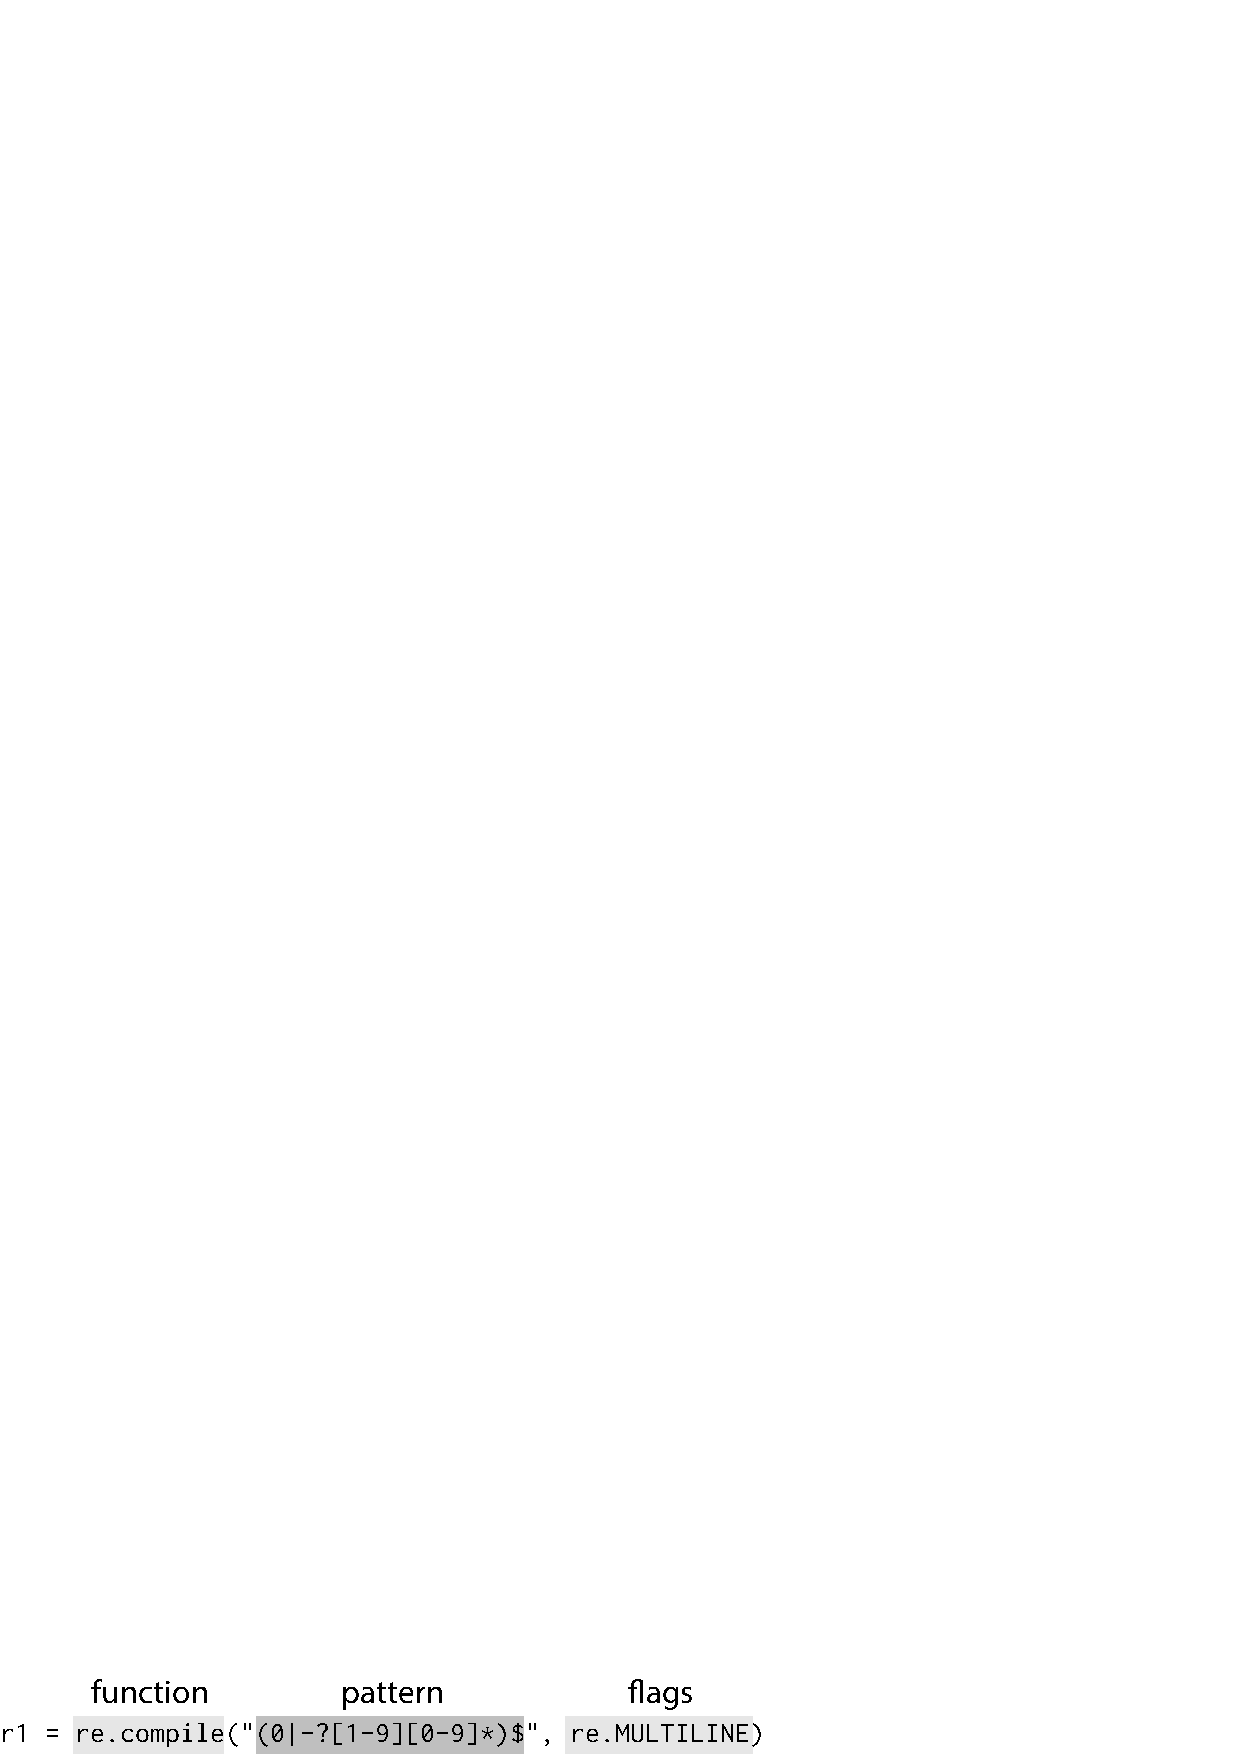
\includegraphics[scale=0.77]{../nontex/illustrations/exampleUsageLarge.pdf}
  \label{fig:exampleUsageLarge}
\end{figure}
\begin{description}
\item [function] which function of the re module is called?
\item [pattern] string used to specify regex behavior
\item [flags] modifies the regex engine
\end{description}
\end{frame}
\note[itemize]{
    \item 53,894 unique utilizations observed.
    \item pt 2
}

